%!TEX root = ../report.tex

\begin{document}
    \chapter{Methodology}
   This section is written in reference to previous work from a colleague and the information obtained from the measX company on to the BMW dataset.

    \section{Data collection setup}
    To monitor proper closing of the car door accelerometer is used which is placed on the door with help of a suction mechanism which can be seen in figure \ref{n1}a. The sensor collects acceleration data in three directions, axis of which are marked in the picture as X to be green, Y as blue and Z as red. The data recording is started before the door bumps into the rubber(marked in red in \ref{n1}b) and stopped when door is still. 
        \begin{figure}[h]
        	\centering
        	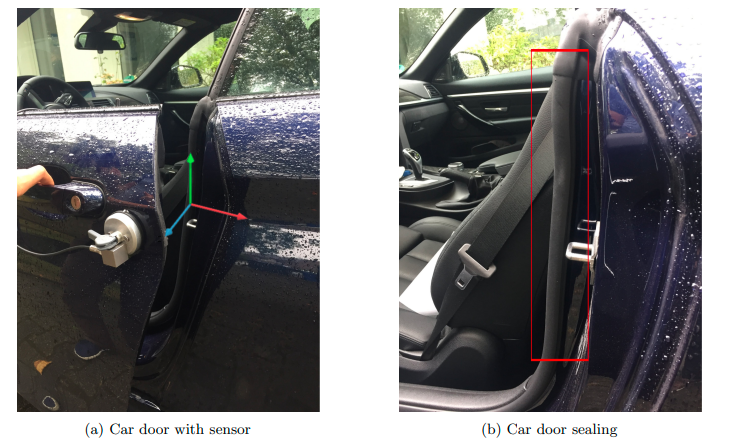
\includegraphics[width=0.9\linewidth]{images/cardoor.png}
        	\caption{Setup for acceleration measurement}
        	\label{n1}
        \end{figure}
        
   The above experiment is carried out for all the four doors of car and six car models. The data collected is labeled according to car model and the door. The recording are stored in Labview format that is TDMS. The reading is 6000ms long which can be seen in \ref{n2}. 
   
   \begin{figure}[h]
   	\centering
   	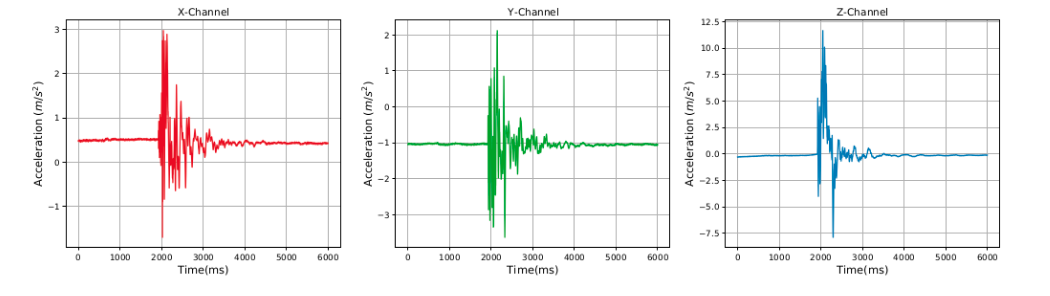
\includegraphics[width=0.9\linewidth]{images/signal.png}
   	\caption{Example of X, Y, Z channels of data}
   	\label{n2}
   \end{figure}
   \section{Data analysis}
   The data collected from sensor is distributed sequentially, that it is a time-series data. As mentioned above there are three channels X, Y and Z. For this experiment the sensor measurements in Z direction are  considered for following reasons:
   
   \begin{itemize}
   	\item There is no motion in X direction as the door of car is hinged.
   	\item The reading in Y direction account for gravity.
   	\item X and Y channels might have false readings due to sensor attached manually.
   	
   	
   \end{itemize}
   
   The data in Z direction is cleaned and downsized to 3500 samples per signal. To analyze the data further and have additional information on to the door closing the acceleration signal is integrated to obtain the velocity and position. Figure \ref{n3} shows example of signal samples of acceleration, velocity and position along Z axis.
   
    \begin{figure}[h]
    	\centering
    	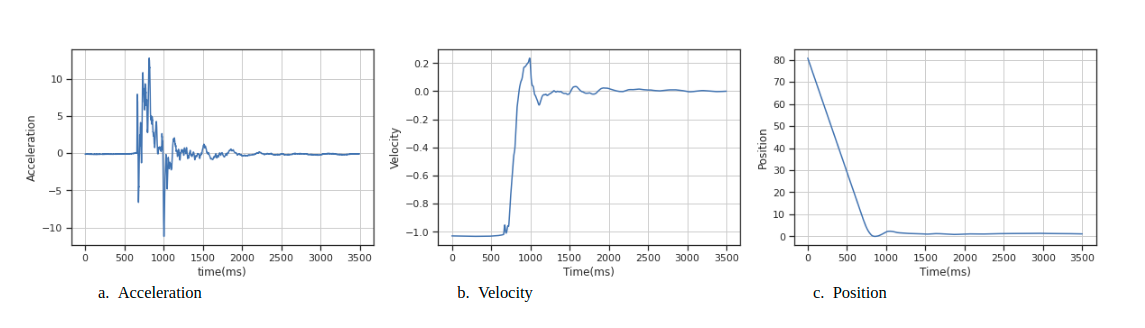
\includegraphics[width=1\linewidth]{images/signalall.png}
    	\caption{Example of acceleration, velocity and position along Z axis}
    	\label{n3}
    \end{figure}
   
  \subsection{Data distribution} 
   The data provided is for six models of BMW cars that can be seen in figure \ref{n4}. As it can be observed from the plot data is highly imbalanced, that is number of negative data samples is very low in comparison to the positive data. 
   
     \begin{figure}[h]
     	\centering
     	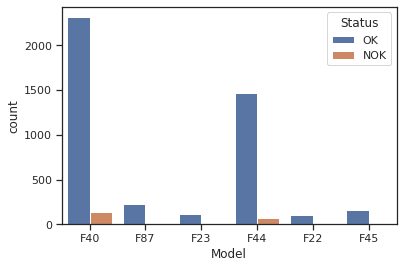
\includegraphics[width=0.6\linewidth]{images/barplot1.png}
     	\caption{Data distribution plot}
     	\label{n4}
     \end{figure}
   
    The signals samples for a positive and negative instance is depicted in figure \ref{n5}. As it can be seen there is no visible difference in the between the instances. This is one of the problems that is addressed in this work.
    
     \begin{figure}[h]
      	\centering
      	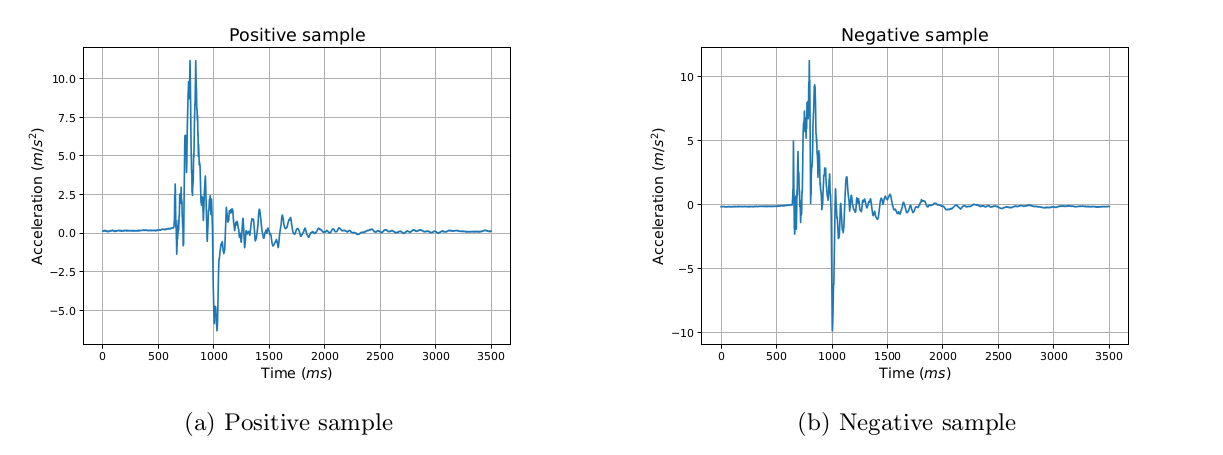
\includegraphics[width=1\linewidth]{images/posneg.png}
      	\caption{Positive and negative samples}
      	\label{n5}
      \end{figure}
      
      
    \section{Manually selected features}
    According to the information provided by the company there are two distinct features maximum velocity and penetration which have been used to classify the data. These features can be visualized in figure \ref{n7}. According the previous work use these features have given better results for classification problem.
    
       \begin{figure}[h]
       	\centering
       	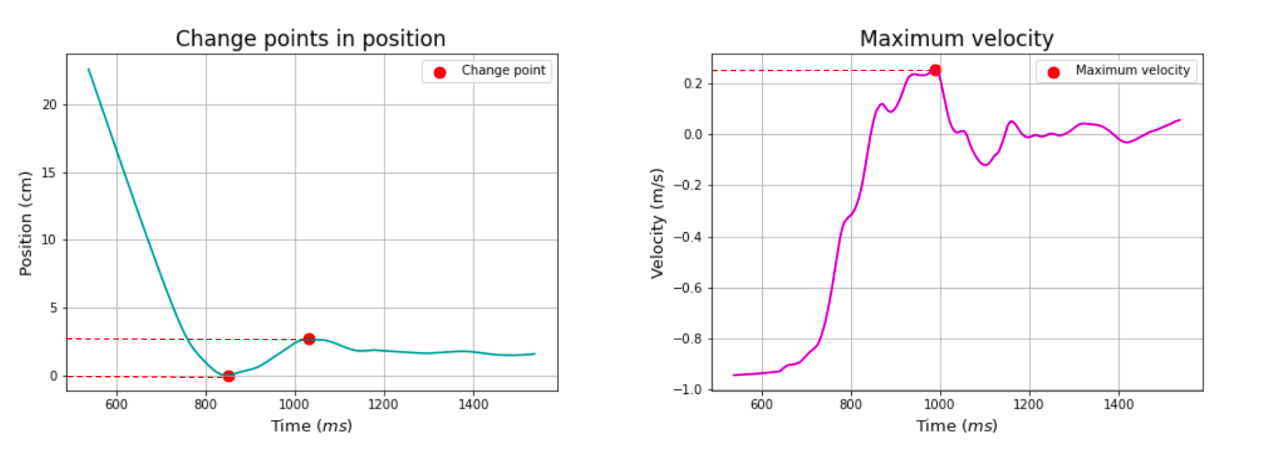
\includegraphics[width=1\linewidth]{images/signal2.png}
       	\caption{Manual features}
       	\label{n7}
       \end{figure}
       
    \section{Data preprocessing}
    \subsection{Data cleaning}
    The data is recorded into LabView TDMS format and a document file with additional information of the maximum velocity and penetration is provided. To simplify the usage important information is selected and saved in pickle format, header of the file can be seen in figure \ref{n8}.
    
     \begin{figure}[h]
     	\centering
     	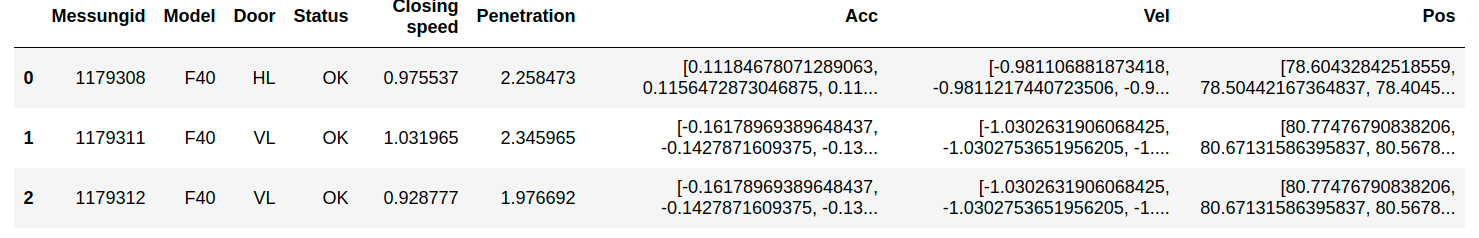
\includegraphics[width=1\linewidth]{images/pickle.png}
     	\caption{Cleaned data file}
     	\label{n8}
     \end{figure}
     
     
    \subsection{Spectrogram}
    As mentioned in sections above we have instances of acceleration velocity and position signal. The spectrograms are generated for each of this instances and sorted according to car model. The generated graph have been stored in image format for analysis. The idea behind using this method is to gain knowledge of both spectral and temporal features and use it as a aid for classification. 
    To generate spectrogram for signal was processed using Fourier analysis. The graph is generated using skit-learn library.
    Example of positive and negative sample spectrogram can be visualized in figure \ref{n9}
    
    \begin{figure}[h]
    	\centering
    	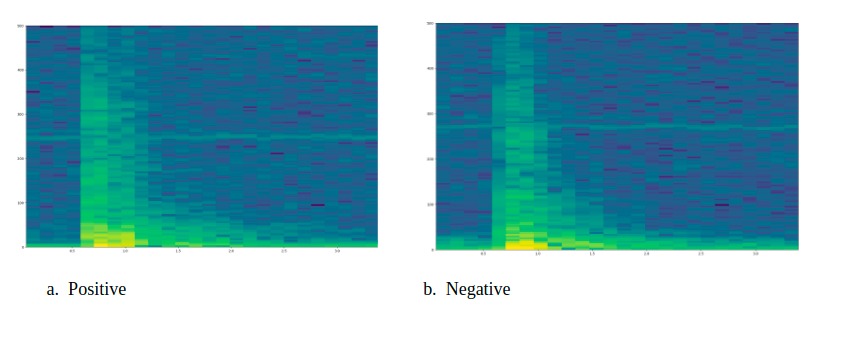
\includegraphics[width=1\linewidth]{images/spec1.png}
    	\caption{Example spectrogram of acceleration signal }
    	\label{n9}
    \end{figure}
  


\end{document}
